\documentclass[11pt]{article}

% the percent sign gives comments in Latex
% top line indicates this is for Physical Review, standard journal format,
% suitable for electronic submission of articles

% the line above is necessary to start any latex document.
% this is one variation that should work for most things.
% if you want double spaceing, use the following:
%
%\documentclass[prd,preprint,letterpaper]{revtex4}
%
% the "preprint" designation will make a wider line
% spacing, good for markup.
\usepackage{graphicx}  % this is the up-to-date package for all figures
\usepackage{float}	% allows use of 'H' command

% these are some custom control of the page size and margins
% \topmargin= 0.2in  % these 1st two may be needed for some computers
%\textheight=8.75in
\textwidth=6.5in
\oddsidemargin=0cm
\evensidemargin=0cm

% this is where the actual document itself (rather than control statements) begins:

\begin{document}

% use a style that gives automatic headings
\pagestyle{myheadings}

% the \title{} command generates a title.

% the \\ below is used to FORCE a line break in the middle of the sentence--
% otherwise latex computes it for you

\title{Lab 4:\\
Random Walks}


\author{Corey Mutnik \\
{\it Computational Physics 305, University of Hawaii at Manoa} }


\date{February 10, 2015}




\maketitle    % this line is necessary to tell latex you are done with all
	      % of the stuff associated with the title, and now it can go
              % ahead and generate the title portion


	      % \section is used to start a new one with a heading
\abstract{

The problem of random walks crops up throughout all of life.  A prime example is brownian motion: the motion of
particles suspended in a solution.  This motion seems random to an observer.  Upon further inspection one realizes 
this motion to be a result of the forces acting on each particle.  Gravitational attraction pulls each particle 
towards the center of our planet.  Various other forces, such as the Coulomb force between particles, also 
play a role in the overall motion that is observed.  Just like the motion itself, computers are unable to generate
genuinely random results.  Using various commands allows for the generation of pseudo-random numbers.  This is done 
using an algorithm that produces results based on the inital input, also called the 'seed'.  Each apparently random 
number generated by our program will always be generated if the same seed number is used.

}

\section{Introduction}

This weeks lab pertained to the apparent random motion of various things in everyday life.  Since computers are 
deterministic machines, they are unable to generate truly random numbers.  Rather, we use commands such as 
'drand48()' to have the computer generate a pseudo-random number.  Starting from a common seed value will always 
output the same results.  Therefore, results are reproducable rather than truly random. 



% one or more lines of space between paragraphs determines them
\section{Code}

The code for this weeks can be seen online: \\
http://www2.hawaii.edu/~cmutnik/lab4.html


\section{Computational problem}

Initally the program generated an uncorrelated set of coordinates.  The independence of these x, y pairs 
was resolved by first defining a randomly generated angle that would be used in the computation of both variables.  
We also bounded the motion from one step to the next by restricting each jump to a length of one unit step.  The 
number of steps taken was graphed against the distance each generated coordinate was from the origin.


    \subsection{Relevant equations}

The errors used in generating figures 1-6 were generated using:
\begin{equation}
\label{F}
 {r[i] \sqrt{Ntrials} \over (Ntrials)^{2}}
\end{equation}


\section{Graphs}

\begin{figure}[H]
  \begin{center}
\centerline{\includegraphics[width=3.75in]{walk_100_10000.png}}
\caption{\it \small{Random Path using Ntrials=100 and Nmax=10,000 \label{fig1}}}
  \end{center}
\end{figure}

\begin{figure}[H]
  \begin{center}
\centerline{\includegraphics[width=3.75in]{walk_100_100000.png}}
\caption{\it \small{Random Path using Ntrials=100 and Nmax=100,000 \label{fig4}}}
  \end{center}
\end{figure}

\begin{figure}[H]
  \begin{center}
\centerline{\includegraphics[width=3.75in]{walk_10_10000.png}}
\caption{\it \small{Random Path using Ntrials=10 and Nmax=10,000 \label{fig2}}}
  \end{center}
\end{figure}

\begin{figure}[H]
  \begin{center}
\centerline{\includegraphics[width=3.75in]{walk_10_100000.png}}
\caption{\it \small{Random Path using Ntrials=10 and Nmax=100,000 \label{fig3}}}
  \end{center}
\end{figure}

\begin{figure}[H]
  \begin{center}
\centerline{\includegraphics[width=3.75in]{walk_4_1000.png}}
\caption{\it \small{Random Path using Ntrials=4 and Nmax=1,000 \label{fig5}}}
  \end{center}
\end{figure}

\begin{figure}[H]
  \begin{center}
\centerline{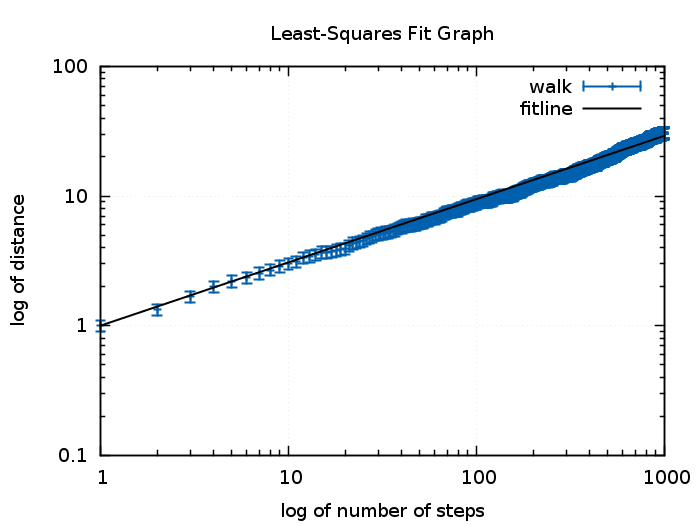
\includegraphics[width=3.75in]{logleastsquaresfit.png}}
\caption{\it \small{Random Path plotted on a logrithmic scale using Ntrials=100 and Nmax=10,000 \label{fig6}}}
  \end{center}
\end{figure}

\begin{figure}[H]
  \begin{center}
\centerline{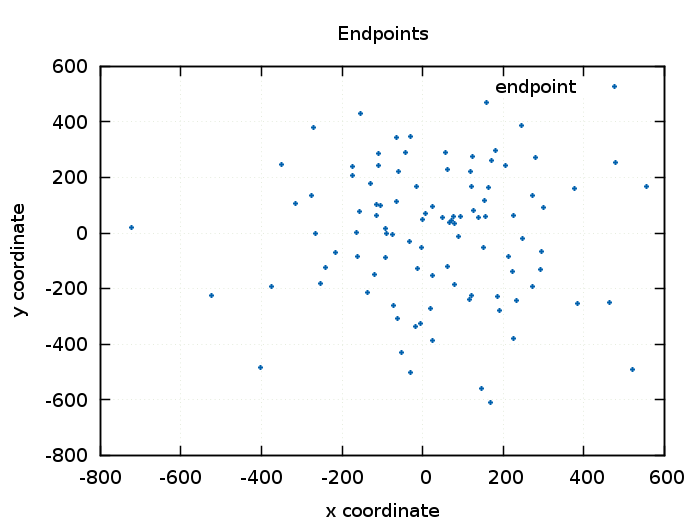
\includegraphics[width=3.75in]{endpoints.png}}
\caption{\it \small{Endpoints using Ntrials=100 and Nmax=10,000 \label{fig7}}}
  \end{center}
\end{figure}

\begin{figure}[H]
  \begin{center}
\centerline{\includegraphics[width=3.75in]{walkpath.png}}
\caption{\it \small{Path of two dimensional random walk \label{fig8}}}
  \end{center}
\end{figure}


\section{Analysis}

Figures 1-6 showed the number of steps graphed against the distance each new coordinate was from the origin, along 
with a best fit line.  Both reducing the number of trials and increasing the maximum number of steps causes the 
error to increase.  This is demonstrated by equation 1 and shown by compairing various figures.  The fitted 
exponent converges to 0.5 at a quicker rate, as the number of trials increases.

Figure 7 is a scatter plot of the endpoints of each trial in two dimensions.  As expected, this graph has a 
distribution that is most dense at the original, approaching an overall even distribution.  Since each unit step 
was taken using a random angle in any direction some steps would be in the opposite direction of the overall motion.  
These steps, occuring less frequently than those that followed the trend, would cause a decrease in the distance 
from the origin from one step to the next.  For this reason it is expected that the uniformity of the scatter plot 
would mimic figure 7.


\section{Conclusion}

It may be impossible for computers to generate truly random numbers but using large prime seeds allowed 
this program to output coordinates with seemingly zero coorelation to each subsequent set.  The generation 
of pseudo-random numbers is extremely benefitial in modeling certian behaviors.  There was a significant 
difference between how long it took to compile the data from paths containing different Ntrial values.  
As the number of steps increased so did the time necessary to compute and collect the data.


\section{Extra Credit}

\begin{figure}[H]
  \begin{center}
\centerline{\includegraphics[width=3.75in]{walkpath3d1.png}}
\caption{\it \small{Three Dimensional Random Walk for three paths - 100, 1,000, and 10,000 steps \label{fig7}}}
  \end{center}
\end{figure}

Figure 8 shows the walk path in 2 dimensions for a single path.  Figure 9 shows the 3-dimensional walk path for
three seperate paths.  The path in red represents one containing 100 steps.  The path in blue represents one 
containing 1,000 steps.  The path in green represents one containing 10,000 steps.

% the following \setlength is to force the bibliography to have no
% paragraph indentations.Can use vairous units--cm are used here.
\setlength{\parindent}{0cm}

\begin{thebibliography}{99}  % the trailing 99 controls some obscure format--just use

\bibitem{Landau} R. H. Landau and M. J. Paez, "Computational Physics, Problem Solving with Computers,"
(Wiley: New York) 1997.

\bibitem{Gorham} P. Gorham, (2014).
\end{thebibliography}

\end{document}

